\pagenumbering{arabic}
%\setcounter{page}{1}
\chapter{Introduction}
\index{Introduction}
\label{sec.matrix}
%start relabeling as 2.1 etc
\pagestyle{myheadings}  \markboth{\ref{sec.matrix}.
\titleref{sec.matrix}}{}
%\setcounter{equation}{0}

\section{Basics}

%\subsection{What is Statistics} \label{ssec.defm}\markright{\ref{ssec.defm} \titleref{ssec.defm}}

Intuitively, statistics can be considered the science of uncertainty. Formally,


\begin{definition}[Statistics]	\index{Statistics!Definition}
Statistics is the science of collecting, classifying, summarizing, analyzing and interpreting data.
\end{definition}

When analyzing a set of data, our goal is to
describe characteristics of a group of objects and
make inferences about the group.
Operationally this involves the collection of data through various means and the analysis and interpretation of data.\\

Statistics can be broken down into two broad categories: descriptive statistics and inferential statistics.

\begin{definition}[Descriptive Statistics]	\index{Statistics!Descriptive statistics}
Descriptive statistics are numerical and graphical methods used to analyze, interpret, and represent data.
\end{definition}

\begin{definition}[Inferential Statistics]	\index{Statistics!Inferential statistics}
Inferential statistics use information from a sample to make generalizations about a larger population.
\end{definition}

Only a very cursory introduction to inferential statistics will be given in this chapter. In subsequent chapters, both descriptive statistics and inferential statistics will be discussed in greater detail.\\

It is important to familiarize yourself with the following definitions as they are used frequently in the field of statistics.

\begin{definition}[Population]	\index{Population!Definition}
A (large) group of units that we are interested in studying.
\end{definition}

\begin{definition}[Sample]		\index{Sample!Definition}
A subset of the population.
\end{definition}

\begin{definition}[Unit]
The objects within a sample for which data are collected. This can be a person, a household, a rabbit, a plant, etc.
\end{definition}

\begin{figure}[H]
	\centering
	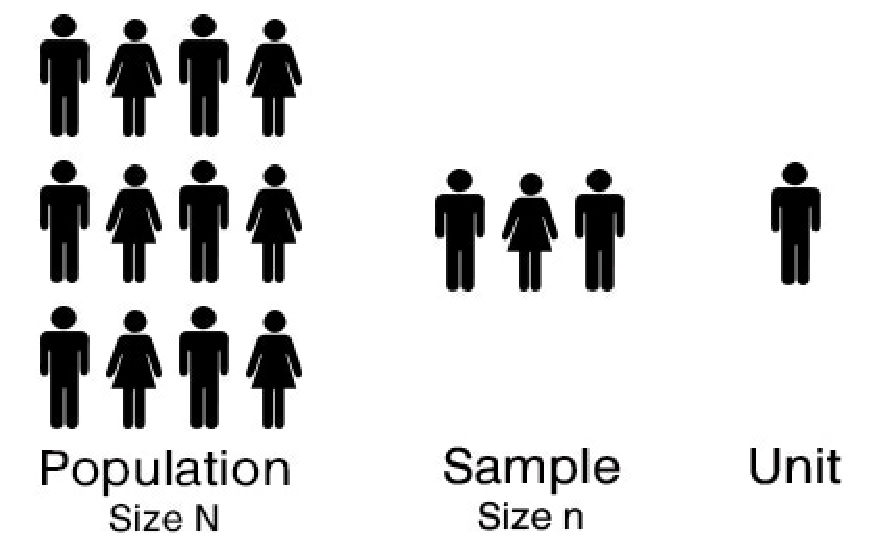
\includegraphics[scale=0.75]{Section1/popsampleunit.pdf}
	\caption{Visualization of the a population, sample and a unit}
\end{figure}

\noindent
Random sampling techniques allow inferences to be drawn on populations and are thus extremely important. The most basic random sample is known as a \textit{simple random sample}.

\begin{definition}[Simple Random Sample]
A simple random sample selects $n$ units from a population with equal probability such that every combination or sample of size $n$ has an equal chance of selection. For a population of size $N$ each unit has a $1/N$ chance of being selected.
\end{definition}

\begin{nt}
More complex sampling techniques include:
	\begin{itemize}\justifying
	\item[-]	Stratified Sampling
	\item[-]	Cluster Sampling
	\item[-]	Multistage Sampling
	\end{itemize}
\end{nt}


\section{Types of Data}	\index{Data!Types of data}

Data can be classified into two main categories: quantitative and qualitative data.

\begin{definition}[Quantitative data]	\index{Data!Quantitative data}
Data that can be measured numerically.
\end{definition}

\noindent
Some examples of quantitative data are:

	\begin{itemize}
	\item	Number of hours you studied this week.
	\item	Distance from your house to the university.
	\item Area (in ft$^{2}$) of the floor of a concourse.
	\end{itemize}


\noindent
Quantitative data can be further divided into discrete data and continuous data.

\begin{definition}[Discrete data]		\index{Data!Discrete data}
Measurements can take only specific values.
\end{definition}

\noindent
Some examples of discrete data are:
	\begin{itemize}
	\item	The number of heads you get when you toss a coin 5 times.
	\item	The number of rooms in a residence.
	\item   The number of 0.5 credit courses a student is currently enrolled.
	\end{itemize}


\begin{definition}[Continuous data]	\index{Data!Continuous data}
Measurements can take any value within a specified range.
\end{definition}

\noindent
Some examples of continuous data are:
\begin{itemize}
	\item Height.
	\item Weight.
	\item The time taken to complete a task.
\end{itemize}

\begin{nt}
Quantitative data can also be categorized as:
\begin{itemize}
\item	Interval data
\item	Ratio data
\end{itemize}
\end{nt}


\begin{definition}[Qualitative data]	\index{Data!Qualitative data}
Data can not be measured numerically and instead falls into categories.
\end{definition}

\noindent
Some examples of qualitative data are:
\begin{itemize}
	\item	Favourite flavour of ice cream.
	\item	Day of the week (Mon, Tue, \ldots) that an event occurred.
	\item	City you live in.
\end{itemize}

\begin{nt}
Qualitative data can be further categorized as:
\begin{itemize}
\item	Nominal data
\item	Ordinal data
\end{itemize}
\end{nt}

\begin{figure}[H]
\centering
	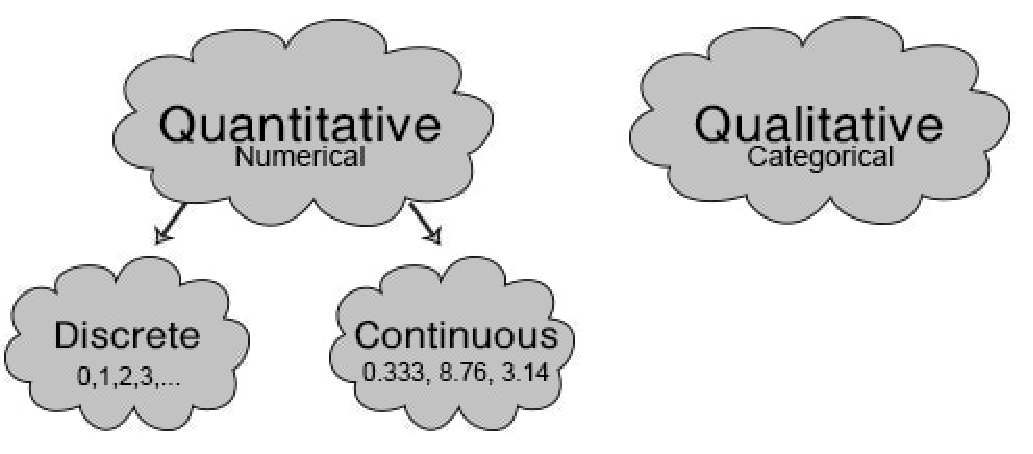
\includegraphics[scale=0.75]{Section1/quantqual.pdf}
		\caption{Simple breakdown of quantitative and qualitative data}
\end{figure}



\section{Types of Studies}

\begin{definition}[Observational Studies]	\index{Studies!Observational studies}
Experimenters observe units and take measurements without assigning treatments.
\end{definition}

In an observational study, we can not decide which units get treatments and which do not. This may be due to ethical reasons or the nature of the study.\\

\noindent
Examples of observational studies include:
\begin{itemize}
\item	The effect of smoking on lung capacity.
\item	The effect of heroin on brain function.
\item	The difference in marks between students who take an in-class course and those who take an online course.
\end{itemize}

\begin{definition}[Experimental Studies]	\index{Studies!Experimental studies}
Treatments are assigned to units and then the effects of the treatment are observed and measured.
\end{definition}

\noindent
In an experimental study we have control over which units do or do not receive a treatment. The group that does not receive a treatment is referred to as the \textit{control group}. A control group is required in experimental studies in order to obtain a baseline for proper statistical comparison.\\

\noindent
Examples of experimental studies include:

	\begin{itemize}
	\item	Testing whether the packaging of a product is appealing to consumers before sending it out to the market.
	\item Providing one group with Windows computers, another (similar) group with Mac computers, and measuring the time taken to complete certain tasks.
	\end{itemize} 

\begin{definition}[Sample surveys]	\index{Sample!Sample surveys}
Data is obtained from a selected part of the population using a survey instrument.
\end{definition}

\noindent
Sample surveys are one of the least expensive types of studies to conduct.\\

\noindent
Some examples of sample surveys include:

\begin{itemize}
\item	Satisfaction survey of guests at a resort.
\item	CSA O-week concert survey.
\end{itemize}


\begin{nt}
Other types of studies include:
	\begin{itemize}
	\item	Case control studies
	\item	Cohort studies
	\item	Cross sectional studies
	\end{itemize}
\end{nt}

\section{Introduction to Inferential Statistics}
\index{Inference!Introduction to inferential statistics}

Before beginning to understand inferential statistics, there are several important definitions that one should become familiar with.

\begin{definition}[Parameter]	\index{Parameter!Definition}
A numerical measure of a population.
\end{definition}

The true value of a parameter is usually \textit{unknown} as it is extremely difficult to take measurements on every unit in a population. The parameters of interest to this course are:

\begin{itemize}
	\item[]	$\mu \>$	 	:	Population mean
	\item[]	$\sigma \>$	:  	Population standard deviation
	\item[]	$p \>$		:  	Population proportion
\end{itemize}

\noindent
The symbols $\mu$ (pronounced ``mew''), $\sigma$ (pronounced ``sigma'') and $p$ are commonly used symbols to represent the population mean, population standard deviation and population proportion respectively.

\begin{definition}[Statistic]		\index{Statistic!Definition}
A numerical measure of a sample.
\end{definition}

Unlike parameters, statistics are \textit{known} values as it is much easier to take measurements on all units in a sample. The statistics of interest to this course are:

\begin{itemize}
	\item	$\bar{x} \>$	: Sample mean
	\item	$s \>$		: Sample standard deviation
	\item	$\hat{p \>}$	: Sample proportion
	\end{itemize}

\noindent
The symbols $\bar{x}$ (pronounced ``$x~bar$''), $s$, and 
$\hat{p}$ (which we call ``$p~hat$'') are 
commonly used symbols to represent the sample mean, 
sample standard deviation and sample proportion respectively.
A statistic is also often referred to as an \textit{estimator}.\\

A conceptual picture of the relationship between population parameters and sample statistics is given in the figure below.

\hfill

\begin{figure}[H]
\begin{center}
\begin{tikzpicture}[scale=1.2]
%\draw[style=dashed] (2,.5) circle (0.5);

\draw[fill=oiB, opacity=0.8] (1,3)
ellipse (3 and 1);

\node[draw=none] at (1,3.25) {Population};
\node[draw=none] at (1,2.60) {$\mu, ~\sigma, ~p$};

\draw[->] (1,2) .. controls (+1.25,1.4) .. (1, 0.75);
\node[draw=none] at (2.50, 1.45) {Draw units};

\draw[fill=oiB7, opacity=0.8] (1,0)
ellipse (2 and 0.7);
\node[draw=none] at (1.00, 0.15) {Sample};
\node[draw=none] at (1,-0.40) {$\bar{x}, ~s, ~\hat{p}$};

%\draw[fill=blue] (0,0) rectangle (1,1);
%\draw[style=thick]
%(3,.5) -- +(30:1) arc(30:80:1) -- cycle;

\end{tikzpicture}
\end{center}
\caption{Conceptual diagram of population, sample, $\mu$, $\sigma$, $\sigma$, 
$\bar{x}$, $s$ and $\hat{p}$.}
\end{figure}

The aim of statistical inference is to produce estimators of the population parameters based on a smaller sample and to
quantify the accuracy of these estimators in terms of a probability statement. 
In other words we are interested in the values of unknown parameters for a population thus we collect data from a sample and calculate statistics to estimate the parameters of interest. We then quantify our confidence that the statistic is representative of the parameter.

\begin{center}
$\bar{x}	\quad	\xrightarrow{\text{Estimate}}	\quad 	\mu$		\\[0.5em]
$s	 	\quad	\xrightarrow{\text{Estimate}}	\quad 	\sigma$	\\[0.5em]
$\hat{p}	\quad	\xrightarrow{\text{Estimate}}	\quad	p$
\end{center}

In business settings, statistics allows us to make informed decisions which \textit{(hopefully)} lead us to most ``profitable`` outcome.
Examples of statistics in business include:%\pause

\begin{enumerate}
\item Data mining%\pause
\item E-commerce%\pause
\item Forecasting%\pause
\item Investment analysis%\pause
\item Marketing%\pause
\item Pricing strategies%\pause
\end{enumerate}



Statistical inference is important in any good decision making process. No matter how one obtains data, data is typically expensive to acquire in terms of time, money and other resources. Sometimes obtaining good data can be very difficult. Furthermore once data is obtained it may need to be cleaned and filtered before it can be used for statistical inference. Once the data is obtained however, 
computation is \textit{cheap} (i.e. not as resource intensive) if the infrastructure is in place. Your value as a statistician (to your employer) will be how you put together the statistical
evidence that will ultimately translate into the profitable outcome.

\section{Issues with Sample Data}

It is usually very difficult (\textit{or impossible}) to measure every unit in a population. It is more feasible and practical to draw a sample and take measurements on all sample units. It is important that the sample be \textit{representative} of the population it is drawn from. This is because we would like to make generalizations about the population based on our sample. In some cases one can control for this using designed experiments or sample surveys. In other cases we do not have control over the sample which is usually the case in observational studies. As a result bias may occur in the sample.
The standard forms of bias are as follows:

\begin{definition}[Selection bias]	\index{Bias!Selection bias}
The sample is not representative of population as a
subset of the population has no chance of being selected for the sample.
\end{definition}

\noindent
An example of selection bias is asking \textit{only} listeners of a left-leaning radio show for their views on the Republican presidential candidate in order to gauge the candidate's nationwide popularity.

\begin{definition}[Non-response bias]		\index{Bias!Non-response bias}
A respondent's refusal to participate may be related to the response variable.
\end{definition}

%\noindent
An example of non-response bias is sampling employees working at a factory in order to determine the effects of a toxic chemical on cancer rates. If an employee has cancer, they would be unable to work and thus would not be included in the sample. Without accounting for this bias it would appear as though the chemicals have little effect.

\begin{definition}[Measurement error bias]		\index{Bias!Measurement error bias}
The response measured and recorded for an individual unit is not correct.
\end{definition}

\noindent
Measurement error bias may occur if study participants misrepresent themselves (e.g. giving a false age or weight) or if measurement tools are improperly calibrated. \\

Ideally we would ideally draw a random sample in order to eliminate 
(or at least minimize) any bias.

\begin{example}
Company ABC is interested in determining the average job satisfaction of all its employees. In order to do so, it distributes a questionnaire to thirty employees working in its IT department. The questionnaire includes the following questions:
\begin{enumerate}
\item How many years have you worked for Company ABC?
\item Is your position at Company ABC full-time or part-time?
\item Rate your overall job satisfaction on a scale of 1-10.
\end{enumerate}

\begin{benumerate}
\item What is the population of interest?
\item[] All employees at Company ABC.
\item What is the sample? 
\item[] Thirty employees working in Company ABC's IT department.
\item Is the data collected quantitative or qualitative? 
\item[] Job satisfaction and length of employment are quantitative as they can be measured numerically. Position status is qualitative as employees can be classified as either full-time or part-time.
\item Is the data discrete or continuous? 
\item[] Job satisfaction is discrete as it can only take on the numbers $1, 2, 3, \hdots, 10$. Length of employment is continuous as it can take on any number such as $1, 2.5, 3.75, \hdots, 24.25$. Position status is qualitative and is therefore neither.
\item What is the parameter of interest? 
\item[] Average job satisfaction of all Company ABC employees.
\item What is the statistic?
\item[] Average job satisfaction of thirty employees working in Company ABC's IT department.
%\item[] Average job satisfaction of thirty employees working in Company ABC’'s IT department.
\item Is this an experimental study, observational study, or sample survey? 
\item[] Sample survey.
\item Is bias present in this sample? 
\item[] Selection bias is present in the selected sample. Only employees in the IT department were surveyed thus employees working in other departments are not represented.
\end{benumerate}

%\hfill\\
%\textbf{\underline{Solutions:}}
%
%\begin{benumerate}
%\item	All employees at Company ABC.
%\item Thirty employees working in Company ABC's IT department.
%\item Job satisfaction and length of employment are quantitative as they can be measured numerically. Position status is qualitative as employees can be classified as either full-time or part-time.
%\item Job satisfaction is discrete as it can only take on the numbers $1, 2, 3, \hdots, 10$. Length of employment is continuous as it can take on any number such as $1, 2.5, 3.75, \hdots, 24.25$. Position status is qualitative and is therefore neither.
%\item Average job satisfaction of all Company ABC employees.
%\item Average job satisfaction of thirty employees working in Company ABC’s IT department.
%\item Sample survey.
%\item	Selection bias is present in the selected sample. Only employees in the IT department were surveyed thus employees working in other departments are not represented.
%\end{benumerate}
\end{example}

\pagebreak

%\bigskip
%\begin{itemize}
%\item[1.] \textbf{selection bias} - sample not representative of population because a
%subset of the population has no chance of being selected for the sample %\pause
%\item[2.] \textbf{nonresponse bias} - respondentsÕ refusals to participate may be related to the response variable %\pause
%\item[3.] \textbf{measurement error bias} - the response measured and recorded for an individual unit is not correct %\pause
%\end{itemize}
%
%
%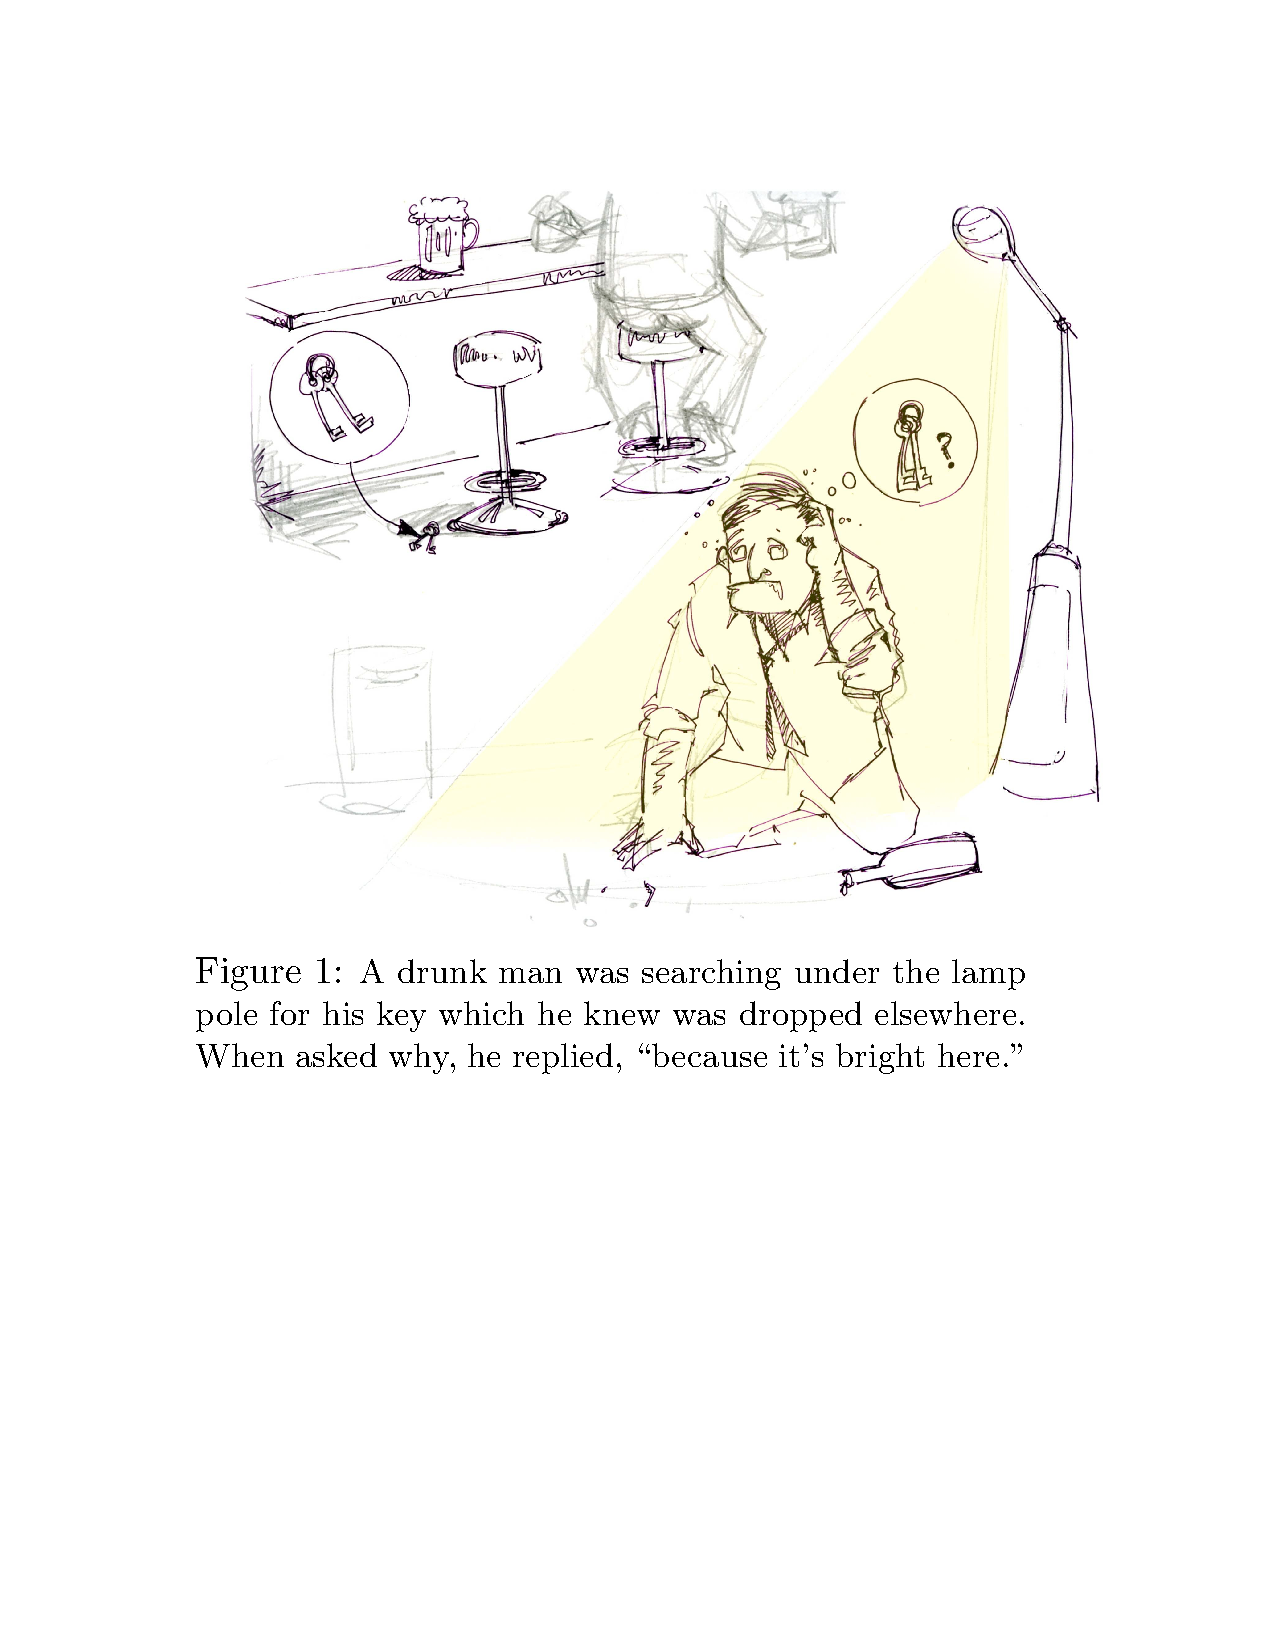
\includegraphics[width=8cm]{Section1/selection_bias}
%
%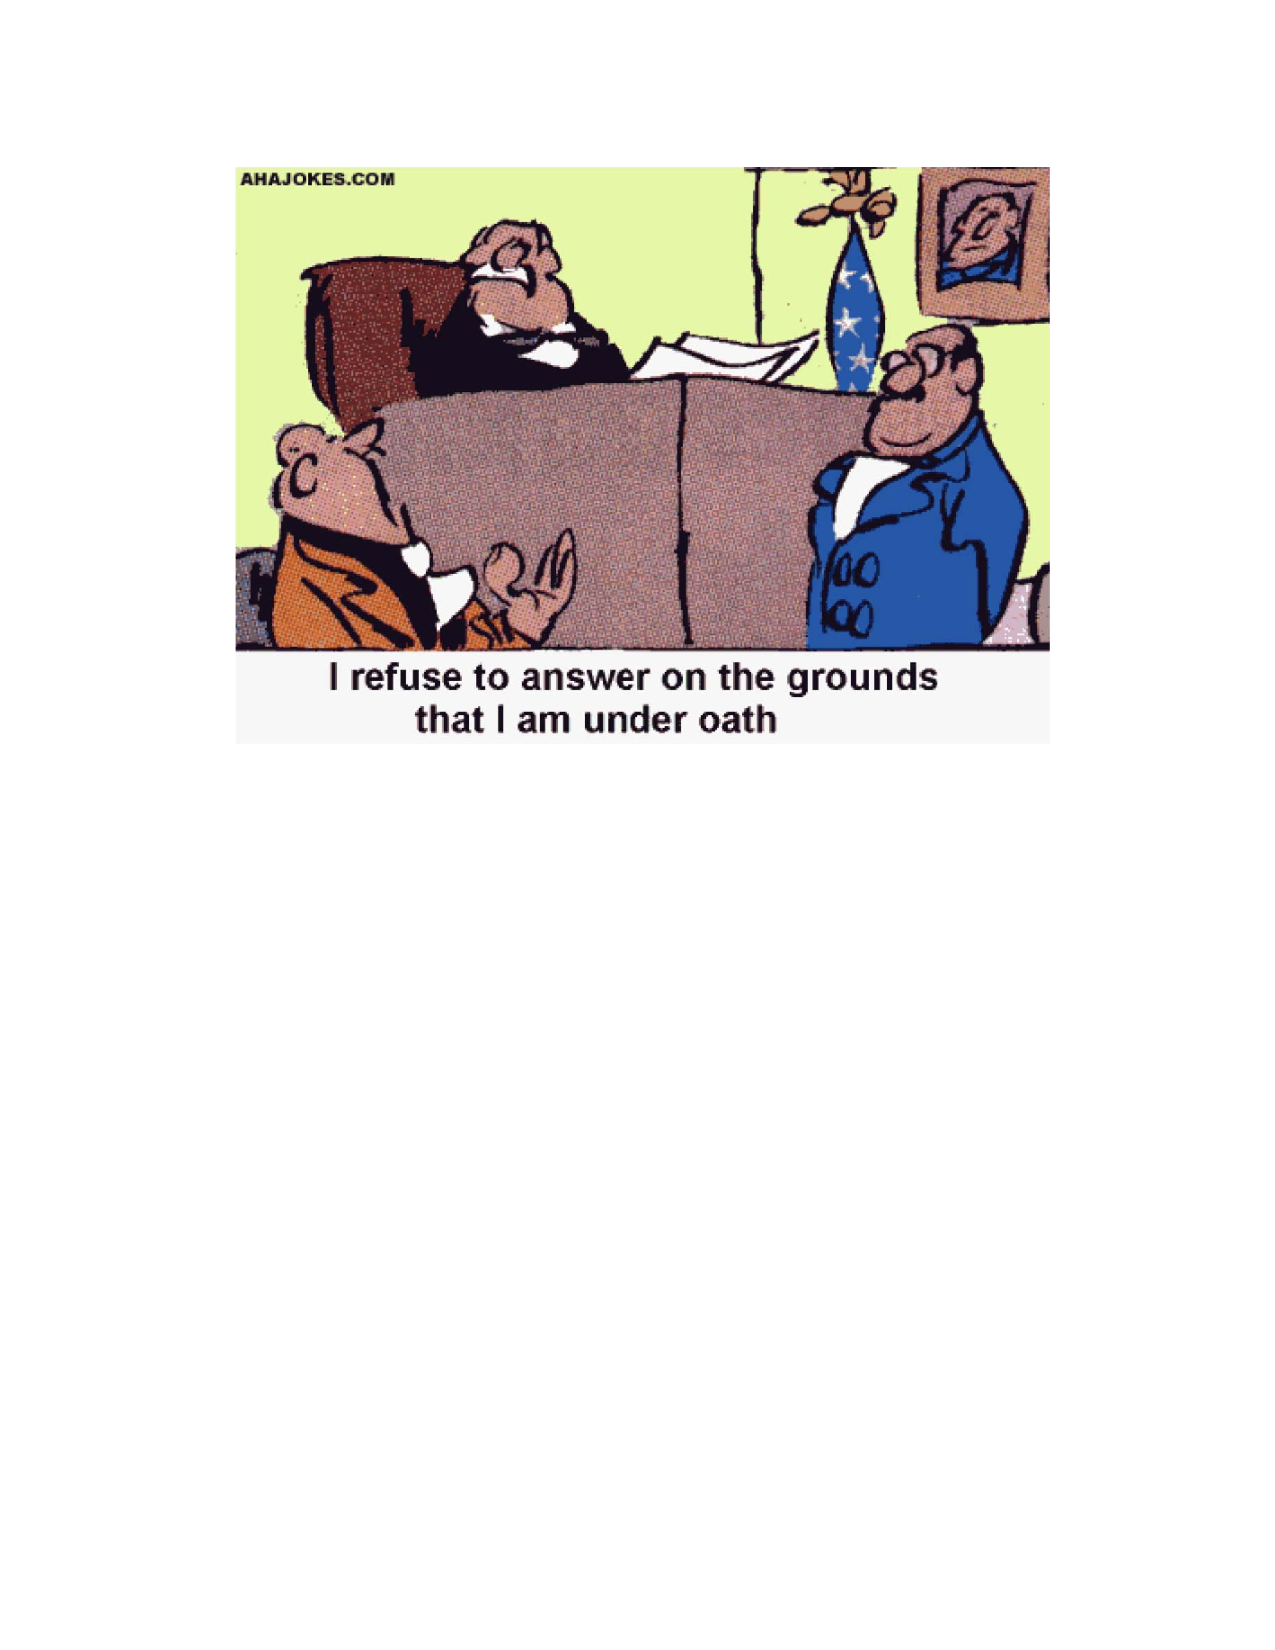
\includegraphics[width=8cm]{Section1/nonresponse_bias}
%
%{\bf On Global Warming:}
%
%\bigskip
%
%``I regret to report that there's no global warming threat after all -- we just got Fahrenheit and Celsius mixed up.''
%
%\bigskip
%
%{\tt www.CartoonStock.com}

%\end{center}

%\section{Plots from our Past}
%
%\subsection{Bar Graphs and Pie Charts}
%
%\textbf{Bar graphs} and \textbf{Pie Charts} are things we should be familiar with.  They are used for
%qualitative data and provides frequencies in each category.
%
%\bigskip
%
%For example, consider the following data concerning inspection at an automobile assembly line.  It was
%determined
%that 70 of  the new cars produced on any given day had the following defects:
%
%
%{\tiny
%\begin{center}
%\begin{tabular}{lrrr}
%Defect&Frequency&Relative Frequency&Relative Frequency (\%)\\ \hline
%Chrome&2&2/70&2.9\\
%Dents&25&25/70&35.7\\
%Paint&30&30/70&42.9\\
%Upholstery&10&10/70&14.3\\
%Windshield&3&3/70&4.3\\ \hline
%\end{tabular}
%\end{center}
%}
%\vspace{-2cm}
%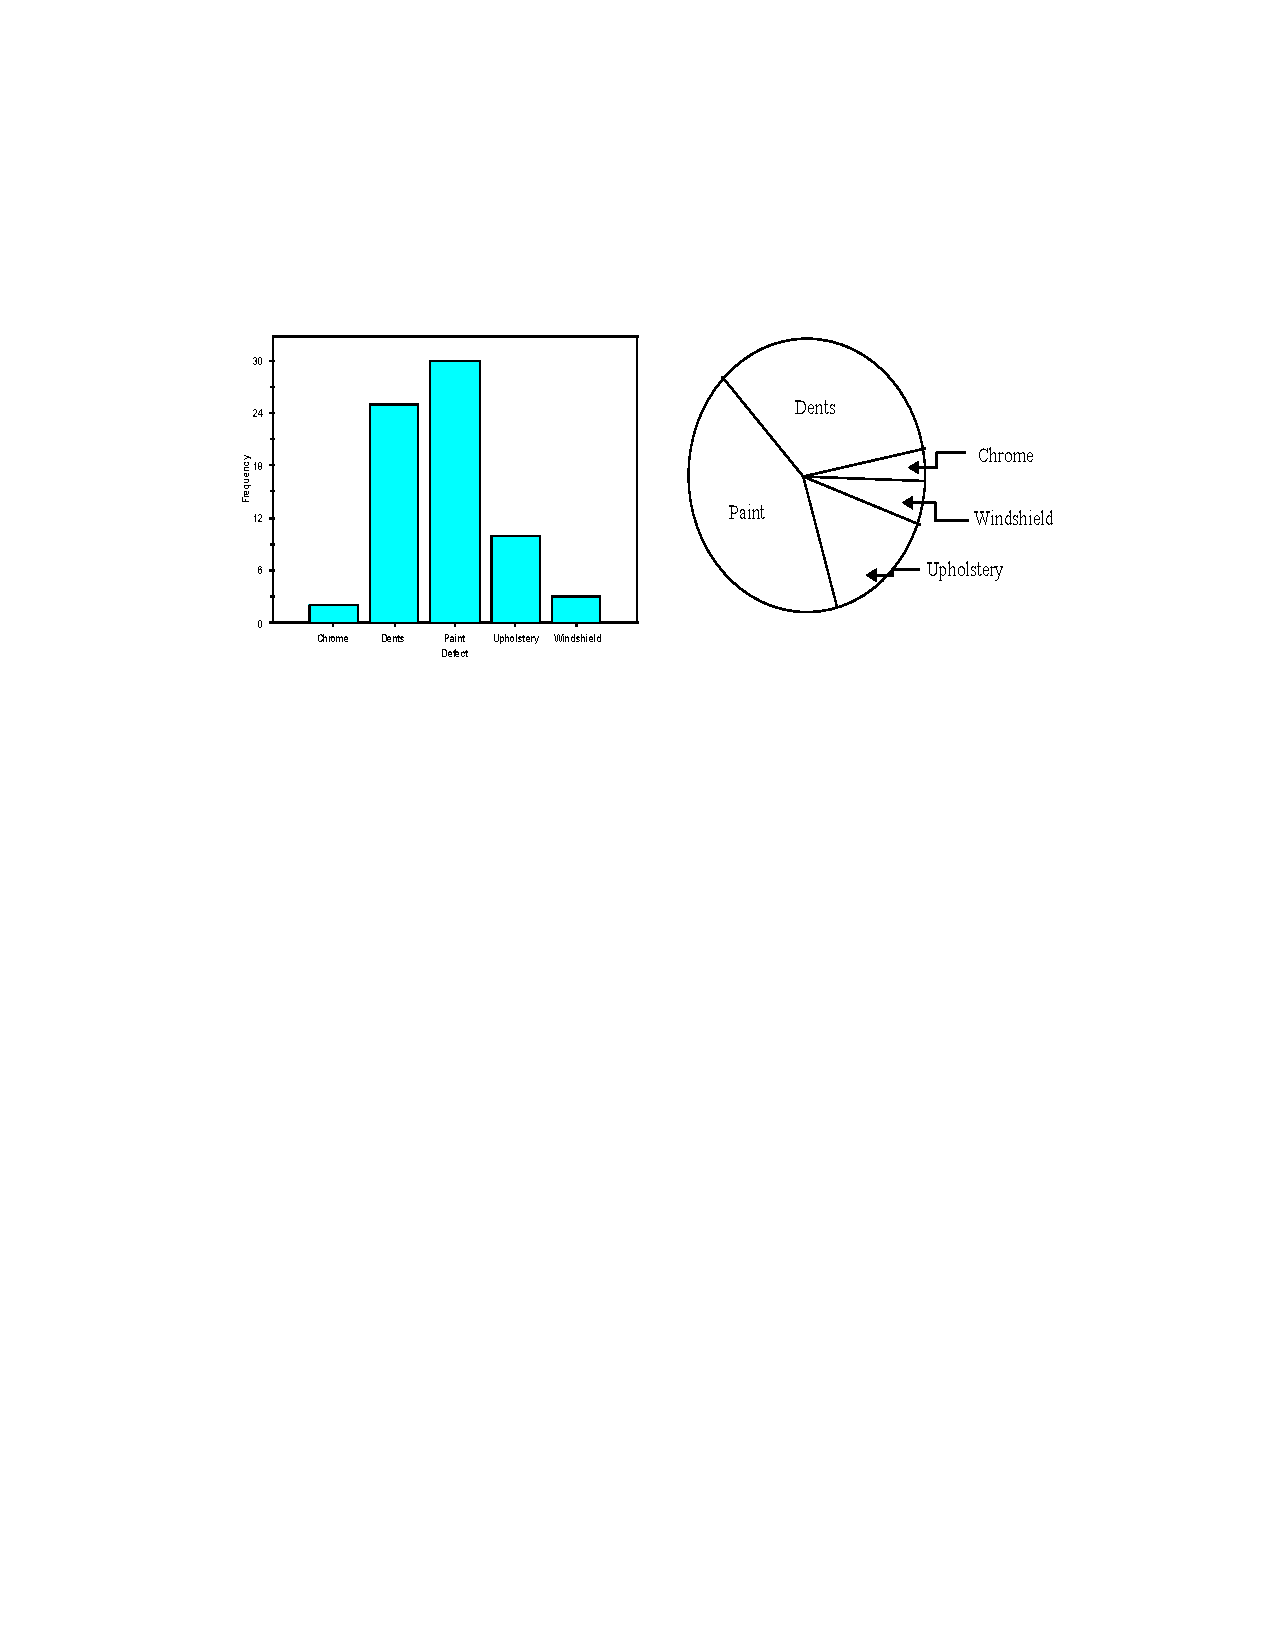
\includegraphics[width=12cm]{Section1/barpie}
%
%\subsection{Histograms and Stemplots}
%
%For quantitative data, there are a number of different plots, the one most
%familiar is a \textbf{histogram}.
%
%\bigskip
%
%This requires one define a \textbf{class} - divide the data into intervals, followed by
%plotting the frequency chart for each class.
%
%\bigskip
%
%For example, consider the delivery time (in days, from order to delivery) for an online
%firm.
%
%\bigskip
%
%32 33 39 43 44 49 49 50 50 51 51 54 56 59 63 64 64 65 68 71 73 82 86 95 102
%
%
%Data:  32 33 39 43 44 49 49 50 50 51 51 54 56 59 63 64 64 65 68 71 73 82 86 95 102
%
%\bigskip
%
%{\tiny
%\begin{center}
%\begin{tabular}{lrrrr}
%Class&Frequency&Relative Frequency&Percentage&Cumulative Frequency\\ \hline
%26--45&5&5/25&20\%&5\\
%46--65&13&13/25&52\%&18\\
%66--85&4&4/25&16\%&22\\
%86--105&3&3/25&12\%&25\\ \hline
%\end{tabular}
%\end{center}
%}
%\vspace{-1cm}
%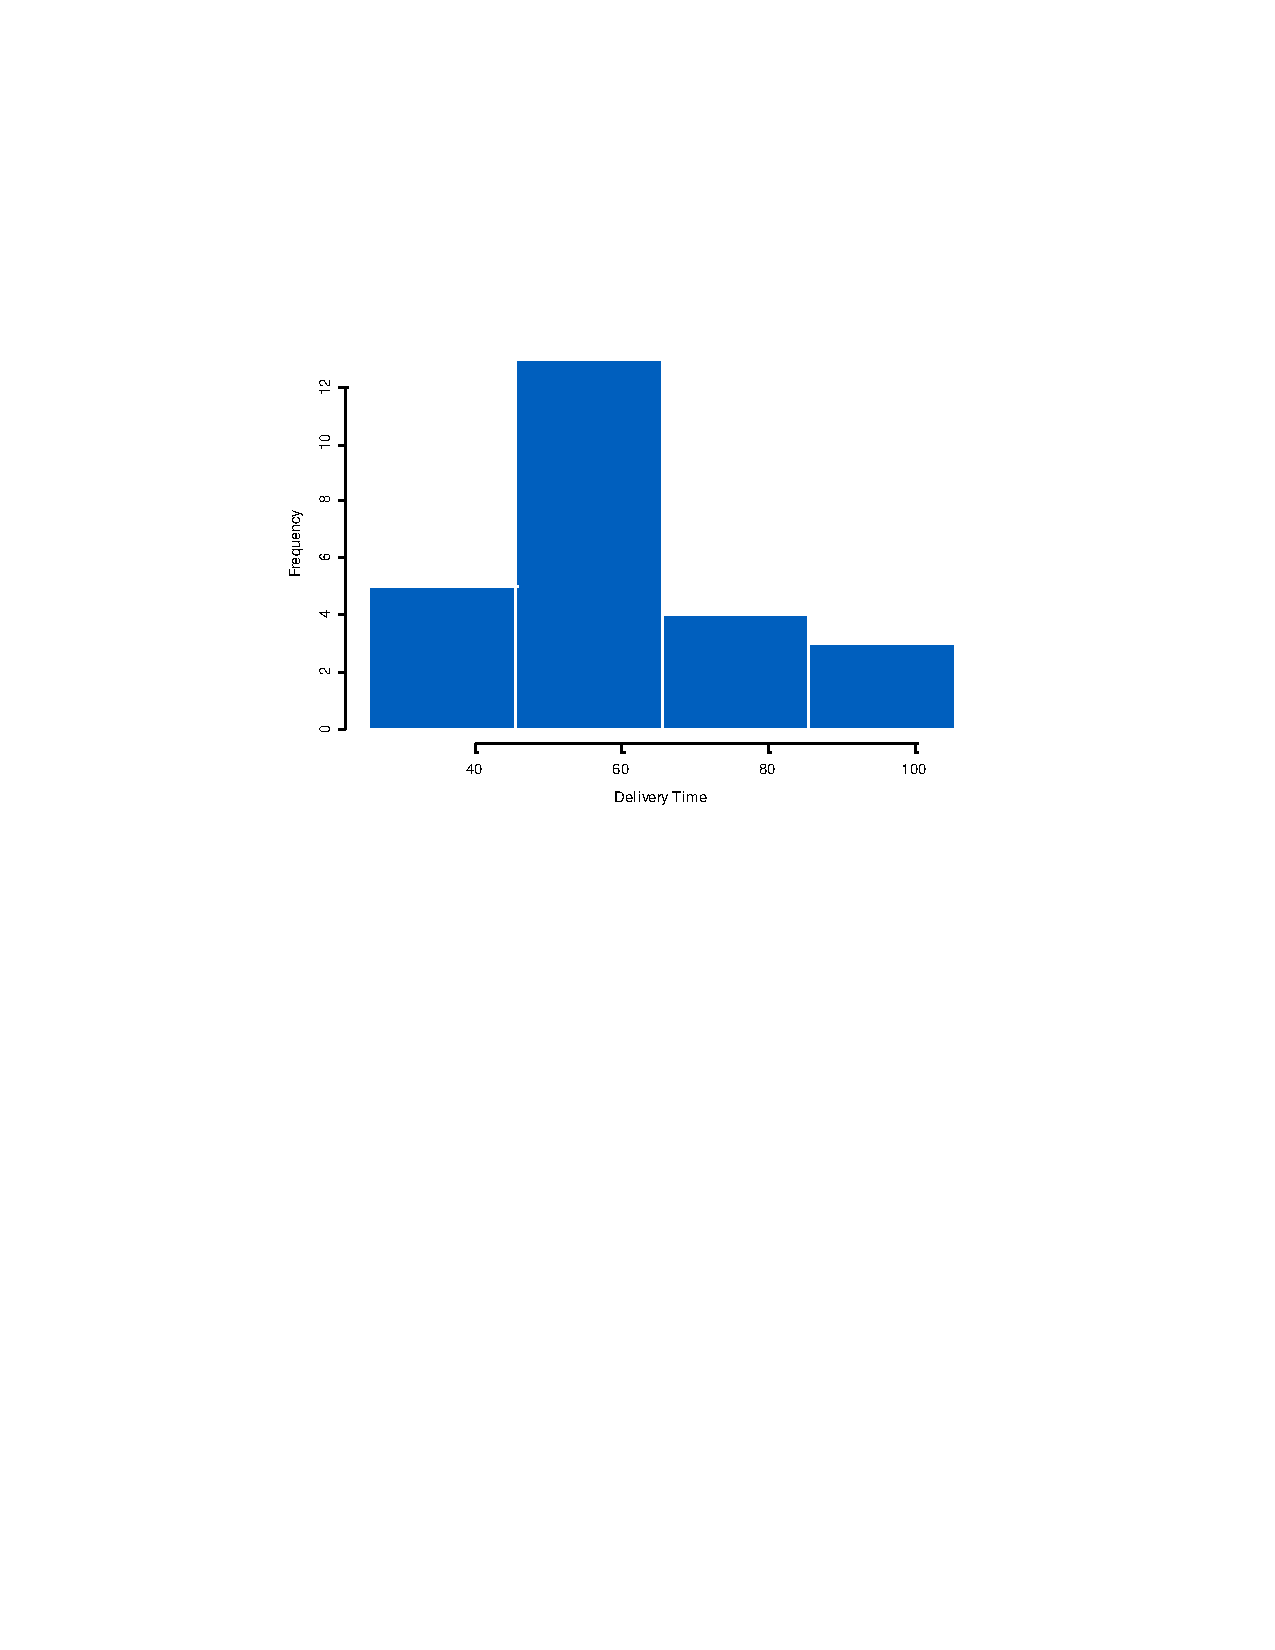
\includegraphics[width=8cm]{Section1/hist-1}
%
%The choice of classes in the table above is somewhat arbitrary. We want to choose enough classes to give us a reasonable picture, but not so many that there are too few observations in each class. The more observations we have, the more classes we can include.
%\vspace{-1cm}
%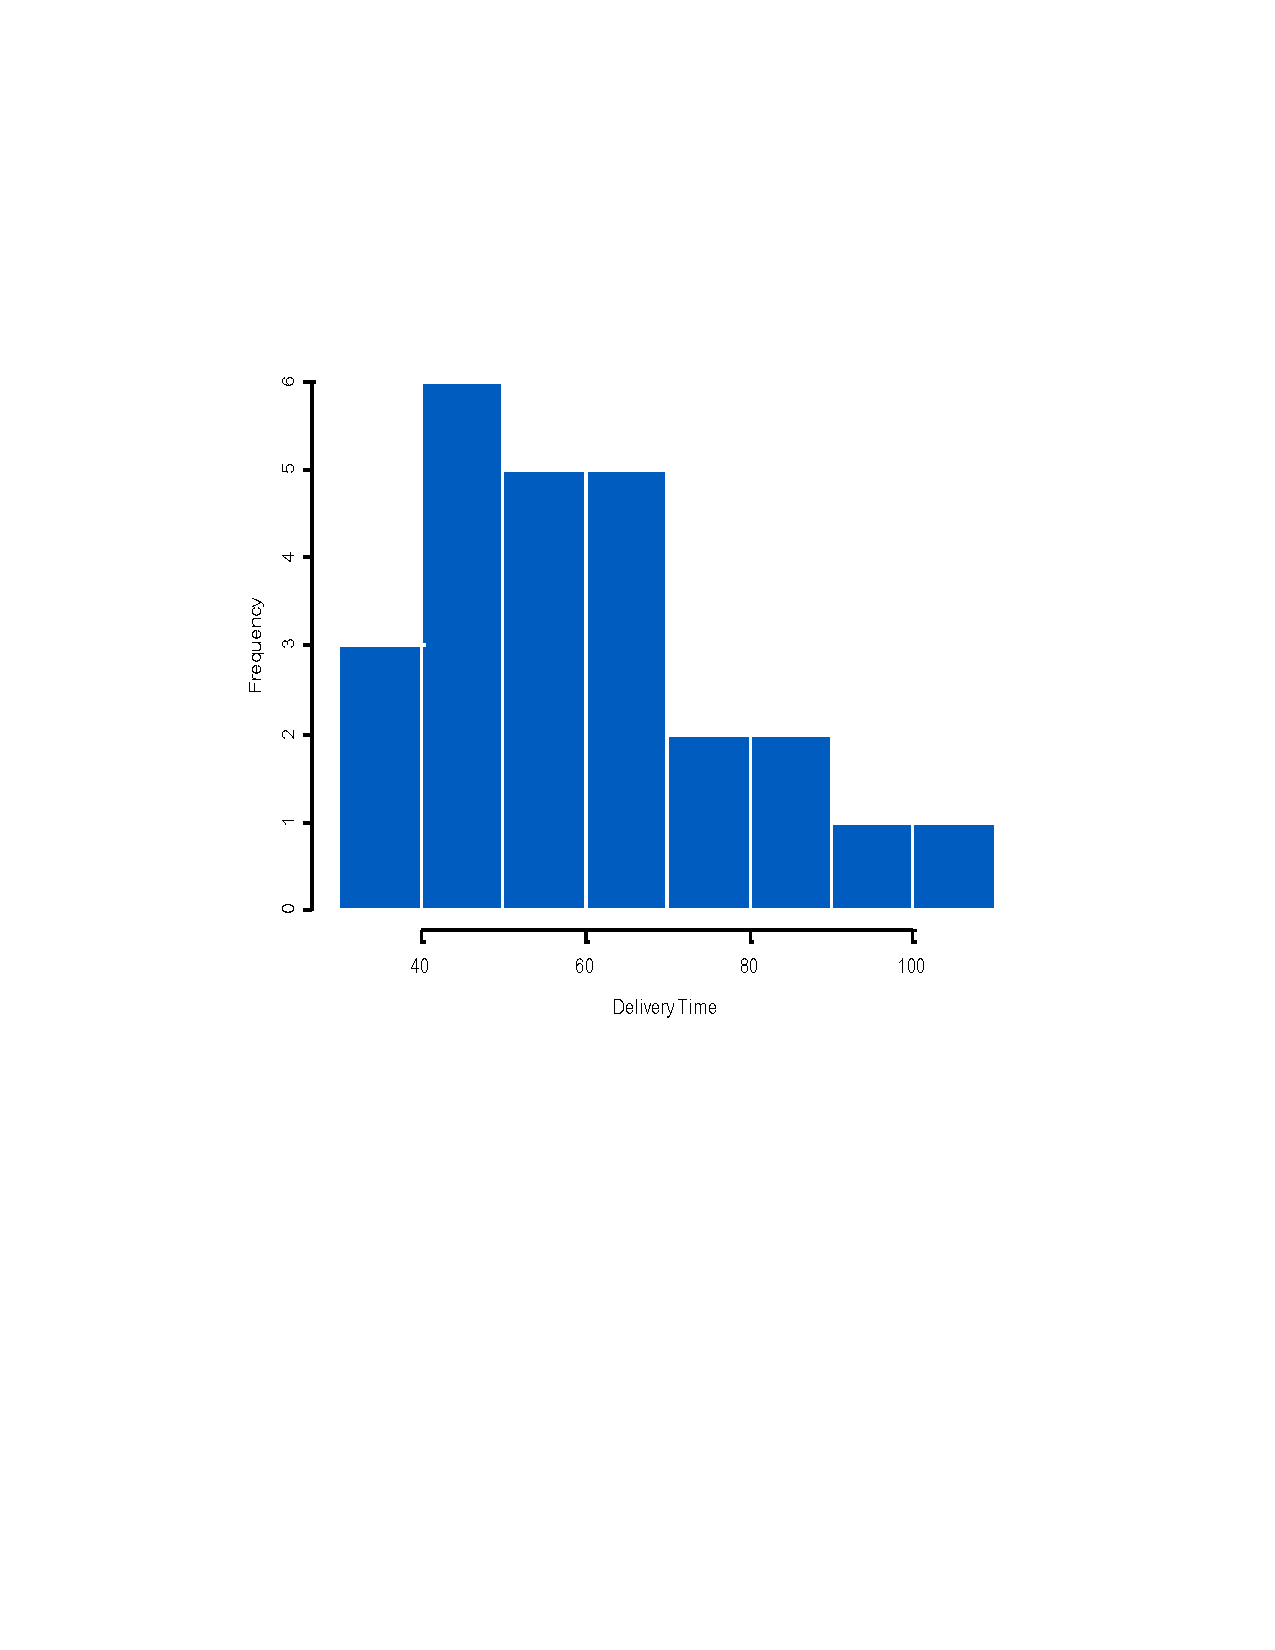
\includegraphics[width=6cm]{Section1/hist-2}
%
%\textbf{Stemplots} are also known as stem-and-leaf plots because each observation (numerical value) is split into a stem and a leaf.
%
%List the stems in a column and write out the leaves next to their corresponding stem.
%
%{\tiny Data:  32 33 39 43 44 49 49 50 50 51 51 54 56 59 63 64 64 65 68 71 73 82 86 95 102}
%
%{\tiny
%\begin{center}
%\begin{tabular}{rl|l}
%Stem&Leaf&Represents the data \ \\ \hline
%3 &239&32 33 39\\
%4 &3499&43 44 49\\
%5 &0011469&50 50 51 51 54 56 59 \\
%6 &34458&63 64 64 65 68 \\
%7 &13&71 73\\
%8 &26&82 86\\
%9 &5&95\\
%10 &2&102\\ \hline
%\end{tabular}
%\end{center}
%}
%
%This is only useful when data sets are small and is not very practical in todays data environment.
%
%The \textbf{distribution} of data tells us what values it takes on, and how often it takes on these values (i.e. the frequencies).
%
%\vspace{-1cm}
%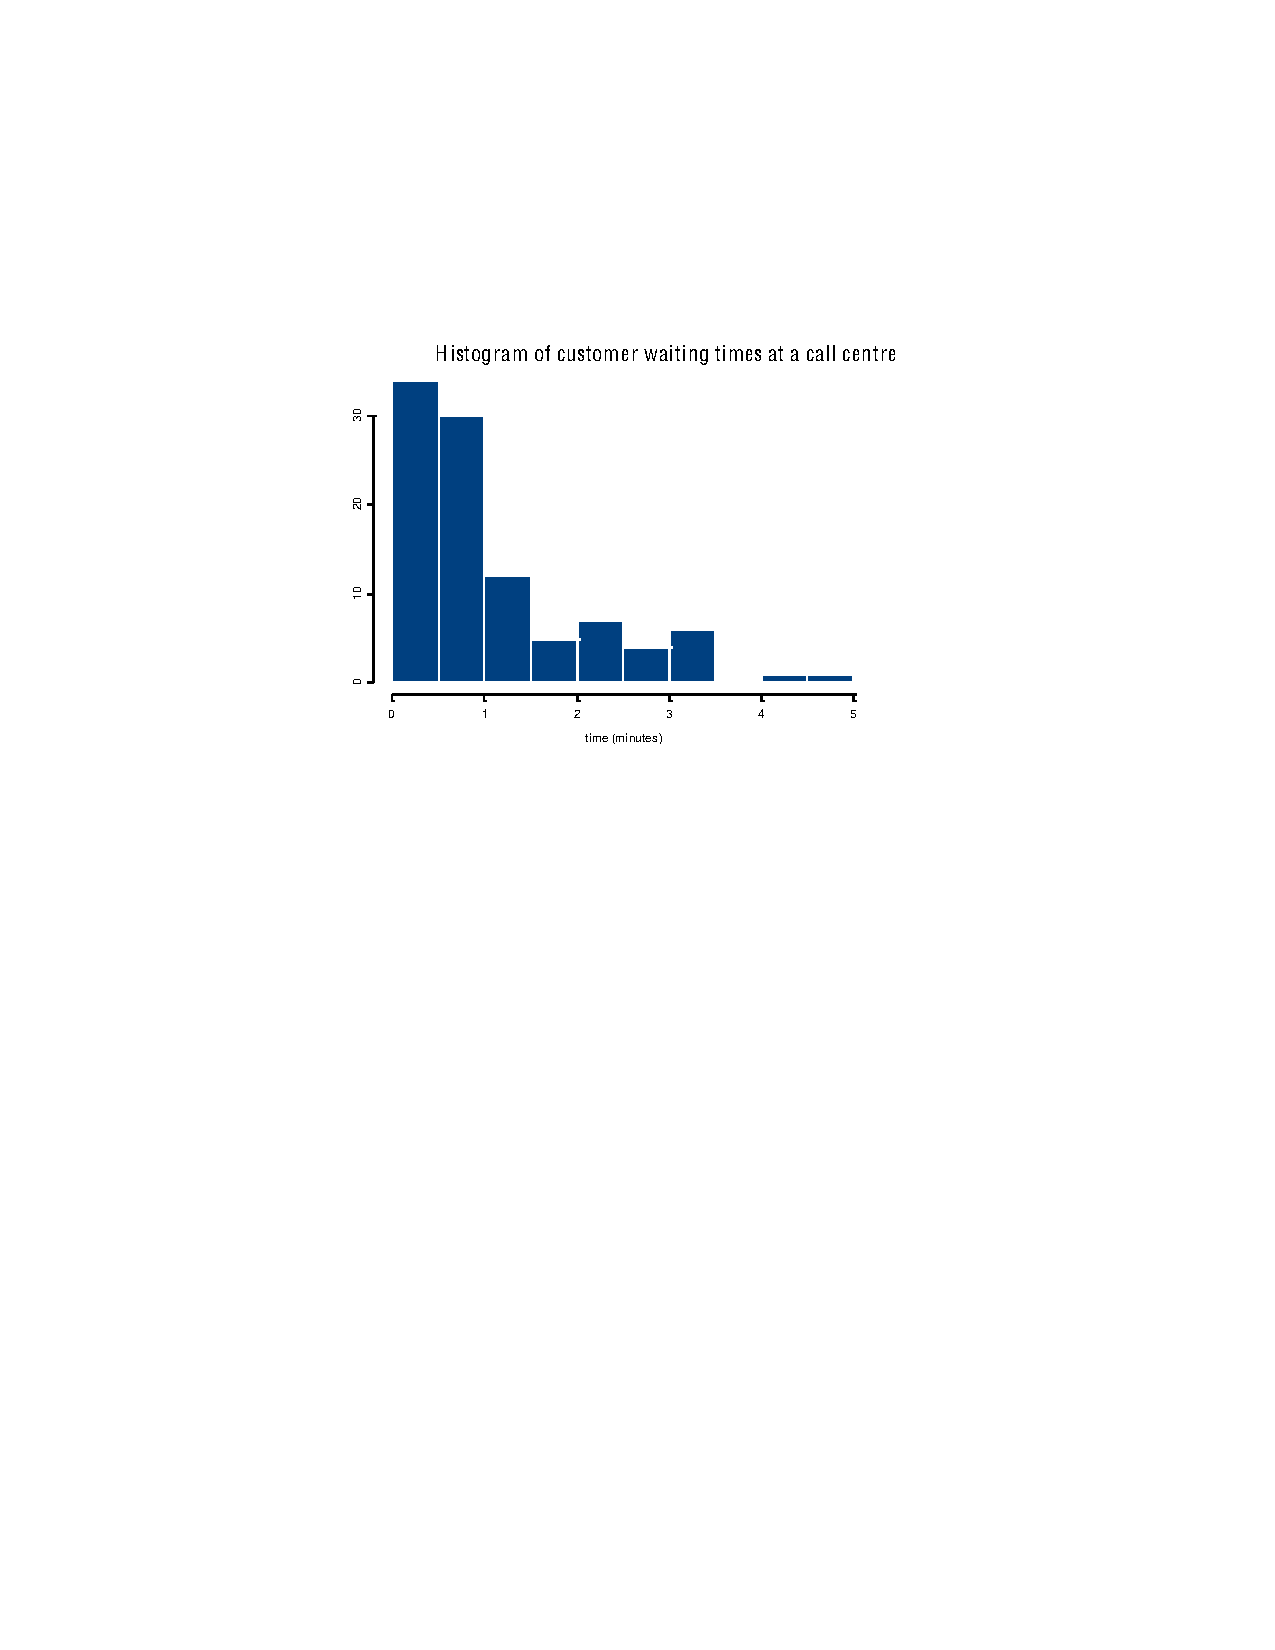
\includegraphics[width=10cm]{Section1/hist-3}
%
%\begin{itemize}
%\item[1.]Where is the centre of the distribution?
%\item[2.]How variable are the observations?
%\item[3.]What is the shape of the distribution?
%Is it symmetric?
%\item[4.]Are there any outliers
%that fall far from the overall pattern?
%\end{itemize}
%
%
%\section{Summary}\label{ssec.sumry2}
%\markright{\ref{ssec.sumry2} \titleref{ssec.sumry2}}
%{\bf Section Keywords: Statistics; Operationally;units;
%population;parameter;sample;
%estimator;qualitative 
%data;quantitative data;observational studies;designed 
%experiments;case controlled studies;sample surveys;random sample; 
%selection bias;
%nonresponse bias;measurement error bias;
%Bar graphs;Pie Charts;histogram;
%class;Stemplots;distribution.}